\documentclass[12pt,aspectratio=169]{beamer}
% \hypersetup{pdfpagemode=FullScreen}

\usepackage{upgreek}
\usefonttheme{professionalfonts}

\renewcommand*{\thefootnote}{\fnsymbol{footnote}}

\mode<presentation>
\useoutertheme[subsection=false]{miniframes}

\AtBeginSection[]{
  \begin{frame}
  \centering
  \begin{beamercolorbox}[sep=8pt,center,shadow=true,rounded=true]{title}
    \usebeamerfont{title}\insertsectionhead\par%
  \end{beamercolorbox}
  \end{frame}
}

\title{Memory-Efficient Pipeline-Parallel DNN Training}
\author{Deepak Narayanan\inst{3} \and Amar Phanishayee\inst{1} \and Kaiyu Shi\inst{2} \and Xie Chen\inst{2} \and Matei Zaharia\inst{3}}
\institute{\inst{1} Microsoft Research
           \inst{2} Microsoft
           \inst{3} Stanford University}
\date{Presenter: Shiwei Zhang}

\begin{document}
    \beamertemplatenavigationsymbolsempty

    \makeatletter
    \def\beamer@andinst{\\[.1em]}
    \makeatother

    \begin{frame}
        \titlepage
    \end{frame}

    \section{Introduction}

    \begin{frame}
        \frametitle{Pipeline Parallelism}

        DNN models are becoming increasingly large. Traditional model parallelism can either lead to GPU
        under-utilization (inter-layer MP) or high communication overhead (tensor MP).

        Pipelining pushs multiple inputs in sequence through a series of workers that each manage one part of the model,
        achieving both high utilization and good computation-communication overlap. However, existing pipelining
        schemes, \textbf{GPipe} and \textbf{PipeDream}, have their own trade-off between throughput and memory
        footprint.
    \end{frame}

    \begin{frame}
        \frametitle{GPipe}

        \begin{center}
            \vskip -4em
            \includegraphics[page=2,trim=2cm 21.9cm 11cm 1.9cm,clip,scale=1]{pipedream-2bw.pdf}
        \end{center}

        GPipe divides a minibatch into $m$ microbatches that share the same version of parameters. Pipeline flushing is
        required after every $m$ microbatches.
    \end{frame}

    \begin{frame}
        \frametitle{PipeDream}

        \begin{center}
            \vskip -4em
            \includegraphics[page=2,trim=11cm 21.2cm 2cm 1.9cm,clip,scale=1]{pipedream-2bw.pdf}
        \end{center}

        PipeDream introduces multiple weight versions and gradient staleness to maximize throughput. At most $d$ versions
        of weights can present at the same time.

    \end{frame}

    \begin{frame}
        \frametitle{Methods}

        \begin{itemize}
            \setlength{\itemsep}{.8em}
            \item Double-Buffered Weight Updates (2BW) that has both high throughput and low memory footprint
            \item A planing algorithm that yields effective parallelization schemes for many of today's large model
            architectures.
        \end{itemize}
    \end{frame}

    \section{Double-Buffered Weight Updates (2BW)}

    \begin{frame}
        \frametitle{Double-Buffered Weight Updates (2BW)}

        \begin{center}
            \vskip -4em
            \includegraphics[page=3,trim=2cm 21.2cm 2cm 1.9cm,clip,scale=0.8]{pipedream-2bw.pdf}
        \end{center}

        Double-Buffered Weight Updates introduces both $m$ microbatches and 2 weight versions. It uses the same 1F1B
        scheduling as in PipeDream.
    \end{frame}

    \begin{frame}
        \frametitle{PipeDream-Flush}

        \begin{columns}
            \begin{column}{0.5\textwidth}
                The paper also introduces PipeDream-Flush, which is simply GPipe with 1F1B scheduling. It have the same
                semantics as GPipe but has lower memory footprint.
            \end{column}
            \begin{column}{0.5\textwidth}
                \includegraphics[page=4,trim=2cm 19cm 11cm 1.9cm,clip,scale=0.9]{pipedream-2bw.pdf}
            \end{column}
        \end{columns}
    \end{frame}

    \begin{frame}
        \frametitle{Memory footprint Comparison}

        \begin{itemize}
            \setlength{\itemsep}{.8em}
            \item \textbf{GPipe}: $m$ activations of batchsize $B/m$, 1 weight version.
            \item \textbf{PipeDream}: $d$ activations of batchsize $B$, $d$ weight versions.
            \item \textbf{PipeDream-2BW}: $d$ activations of batchsize $B/m$, 2 weight versions.
            \item \textbf{PipeDream-Flush}: $d$ activations of batchsize $B/m$, 1 weight versions.
        \end{itemize}
    \end{frame}

    \begin{frame}
        \frametitle{Semantics Comparison}

        \begin{itemize}
            \setlength{\itemsep}{.8em}
            \item \textbf{GPipe}: $W^{(t+1)} = W^{(t)} - \nu \cdot \nabla f(W^{(t)})$
            \item \textbf{PipeDream}: $W^{(t+1)} = W^{(t)} - \nu \cdot \nabla f(W^{(t-d+1)})$
            \item \textbf{PipeDream-2BW}: $W^{(t+1)} = W^{(t)} - \nu \cdot \nabla f(W^{(t-1)})$
            \item \textbf{PipeDream-Flush}: $W^{(t+1)} = W^{(t)} - \nu \cdot \nabla f(W^{(t)})$
        \end{itemize}
    \end{frame}

    \section{Planner}

    \begin{frame}
        \frametitle{Planner}

        \begin{center}
            \vskip -4em
            \includegraphics[page=5,trim=2cm 21.2cm 2cm 1.9cm,clip,scale=0.7]{pipedream-2bw.pdf}
        \end{center}

        \vskip -.5em
        The planner of PipeDream-2BW is an \textit{exhaustive} searching over a \textit{reduced} space. The strategy
        space is $(w, d, b, r)$:

        \begin{itemize}
            \setlength{\itemsep}{.5em}
            \item $w$: the data parallelism replicas,
            \item $d$: the number of stages,
            \item $b$: the microbatch size,
            \item $r$: boolean whether activations should be recomputed
        \end{itemize}
    \end{frame}

    \begin{frame}
        \frametitle{Cost Model}

        \begin{itemize}
            \setlength{\itemsep}{.8em}
            \item In the experiments, the authors use end-to-end profile-based cost functions.
            \item They also presents a closed form cost function that needs less profiling but provides lower accuracy.
            It use the forward and backward time of each block at different batchsizes to simulate the execution.
        \end{itemize}
    \end{frame}

    \begin{frame}
        \frametitle{Example Configurations}

        \begin{center}
            \includegraphics[page=7,trim=2cm 20.8cm 11cm 1.9cm,clip,scale=1.1]{pipedream-2bw.pdf}
        \end{center}
    \end{frame}

    \section{Evaluation}

    \begin{frame}
        \frametitle{Experiments Setup}

        \begin{itemize}
            \setlength{\itemsep}{.8em}
            \item Hardware: \\ (a) 8 8x V100 (16GB) with NVLink. \\ (b) single machine with 8x V100 (32GB).
            \item Implementation: PyTorch implementation adapted from Megatron.
            \item Models: BERT and GPT with 1.3, 2.2 and 3.9 billions of parameters.
            \item Baselines: Model parallelism (inter-layer MP and tensor MP) and GPipe.
        \end{itemize}
    \end{frame}

    \begin{frame}
        \frametitle{Convergence}

        \begin{center}
            \vskip -2em
            \includegraphics[page=8,trim=11cm 18.8cm 2cm 1.9cm,clip,scale=1]{pipedream-2bw.pdf}
        \end{center}
    \end{frame}

    \begin{frame}
        \frametitle{Throughput}

        \begin{center}
            \vskip -1em
            \includegraphics[page=9,trim=2cm 16.1cm 2cm 2cm,clip,scale=0.78]{pipedream-2bw.pdf}
        \end{center}
    \end{frame}

    \begin{frame}
        \frametitle{Throughput cont'd}

        \begin{itemize}
            \setlength{\itemsep}{.8em}
            \item 16-way Tensor MP requires cross-server all-to-all communication in each layer.
            \item GPipe's high memory footprint limits its maximum $m$, which causes large bubbles in the pipeline.
            \item PipeDream-Flush performs better with high batchsizes. However, batchsizes cannot scale to infinity
            without affecting convergence.
        \end{itemize}
    \end{frame}

    \begin{frame}
        \frametitle{Memory Footprint}

        \begin{center}
            \vskip -1em
            \includegraphics[page=10,trim=2cm 19cm 11cm 2cm,clip,scale=1]{pipedream-2bw.pdf}
        \end{center}
    \end{frame}

    \appendix

    \begin{frame}
        \frametitle{Conclusion}

        \textbf{Summary}

        \vskip .6em
        \begin{itemize}
            \setlength{\itemsep}{.8em}
            \item A new pipelining scheme that combines the high throughput of PipeDream and the low memory footprint
            and staleness of GPipe.
            \item A simple planner to automatically find optimal parallelism configurations.
        \end{itemize}

        \vskip 1em
        \textbf{Limitation}

        \vskip .6em
        \begin{itemize}
            \setlength{\itemsep}{.8em}
            \item It assumes repetitive model structures (therefore stage division is trivial) and homogeneous clusters.
        \end{itemize}

    \end{frame}

    \begin{frame}
        \frametitle{Takeaways}

        \begin{itemize}
            \setlength{\itemsep}{.8em}
            \item Combine two existing methods to build a new method that has the advantages of both.
            \item Simple searching algorithm over carefully designed space.
        \end{itemize}
    \end{frame}

    \begin{frame}
        \vskip 1.5em

        \centering \huge
        Thank you!
    \end{frame}
\end{document}
